\section{Proposed Framework: SHAP-DA-IDS}
\label{sec:methodology}

The proposed \textbf{SHAP-DA-IDS} framework consists of five main steps, shown in Fig.~\ref{fig:architecture}: (1) data cleaning and encoding, (2) SHAP-guided feature selection, (3) empirical class difficulty estimation, (4) difficulty-adaptive augmentation, and (5) classification with post-hoc TreeSHAP explainability.

\begin{figure*}[!t]
\centering
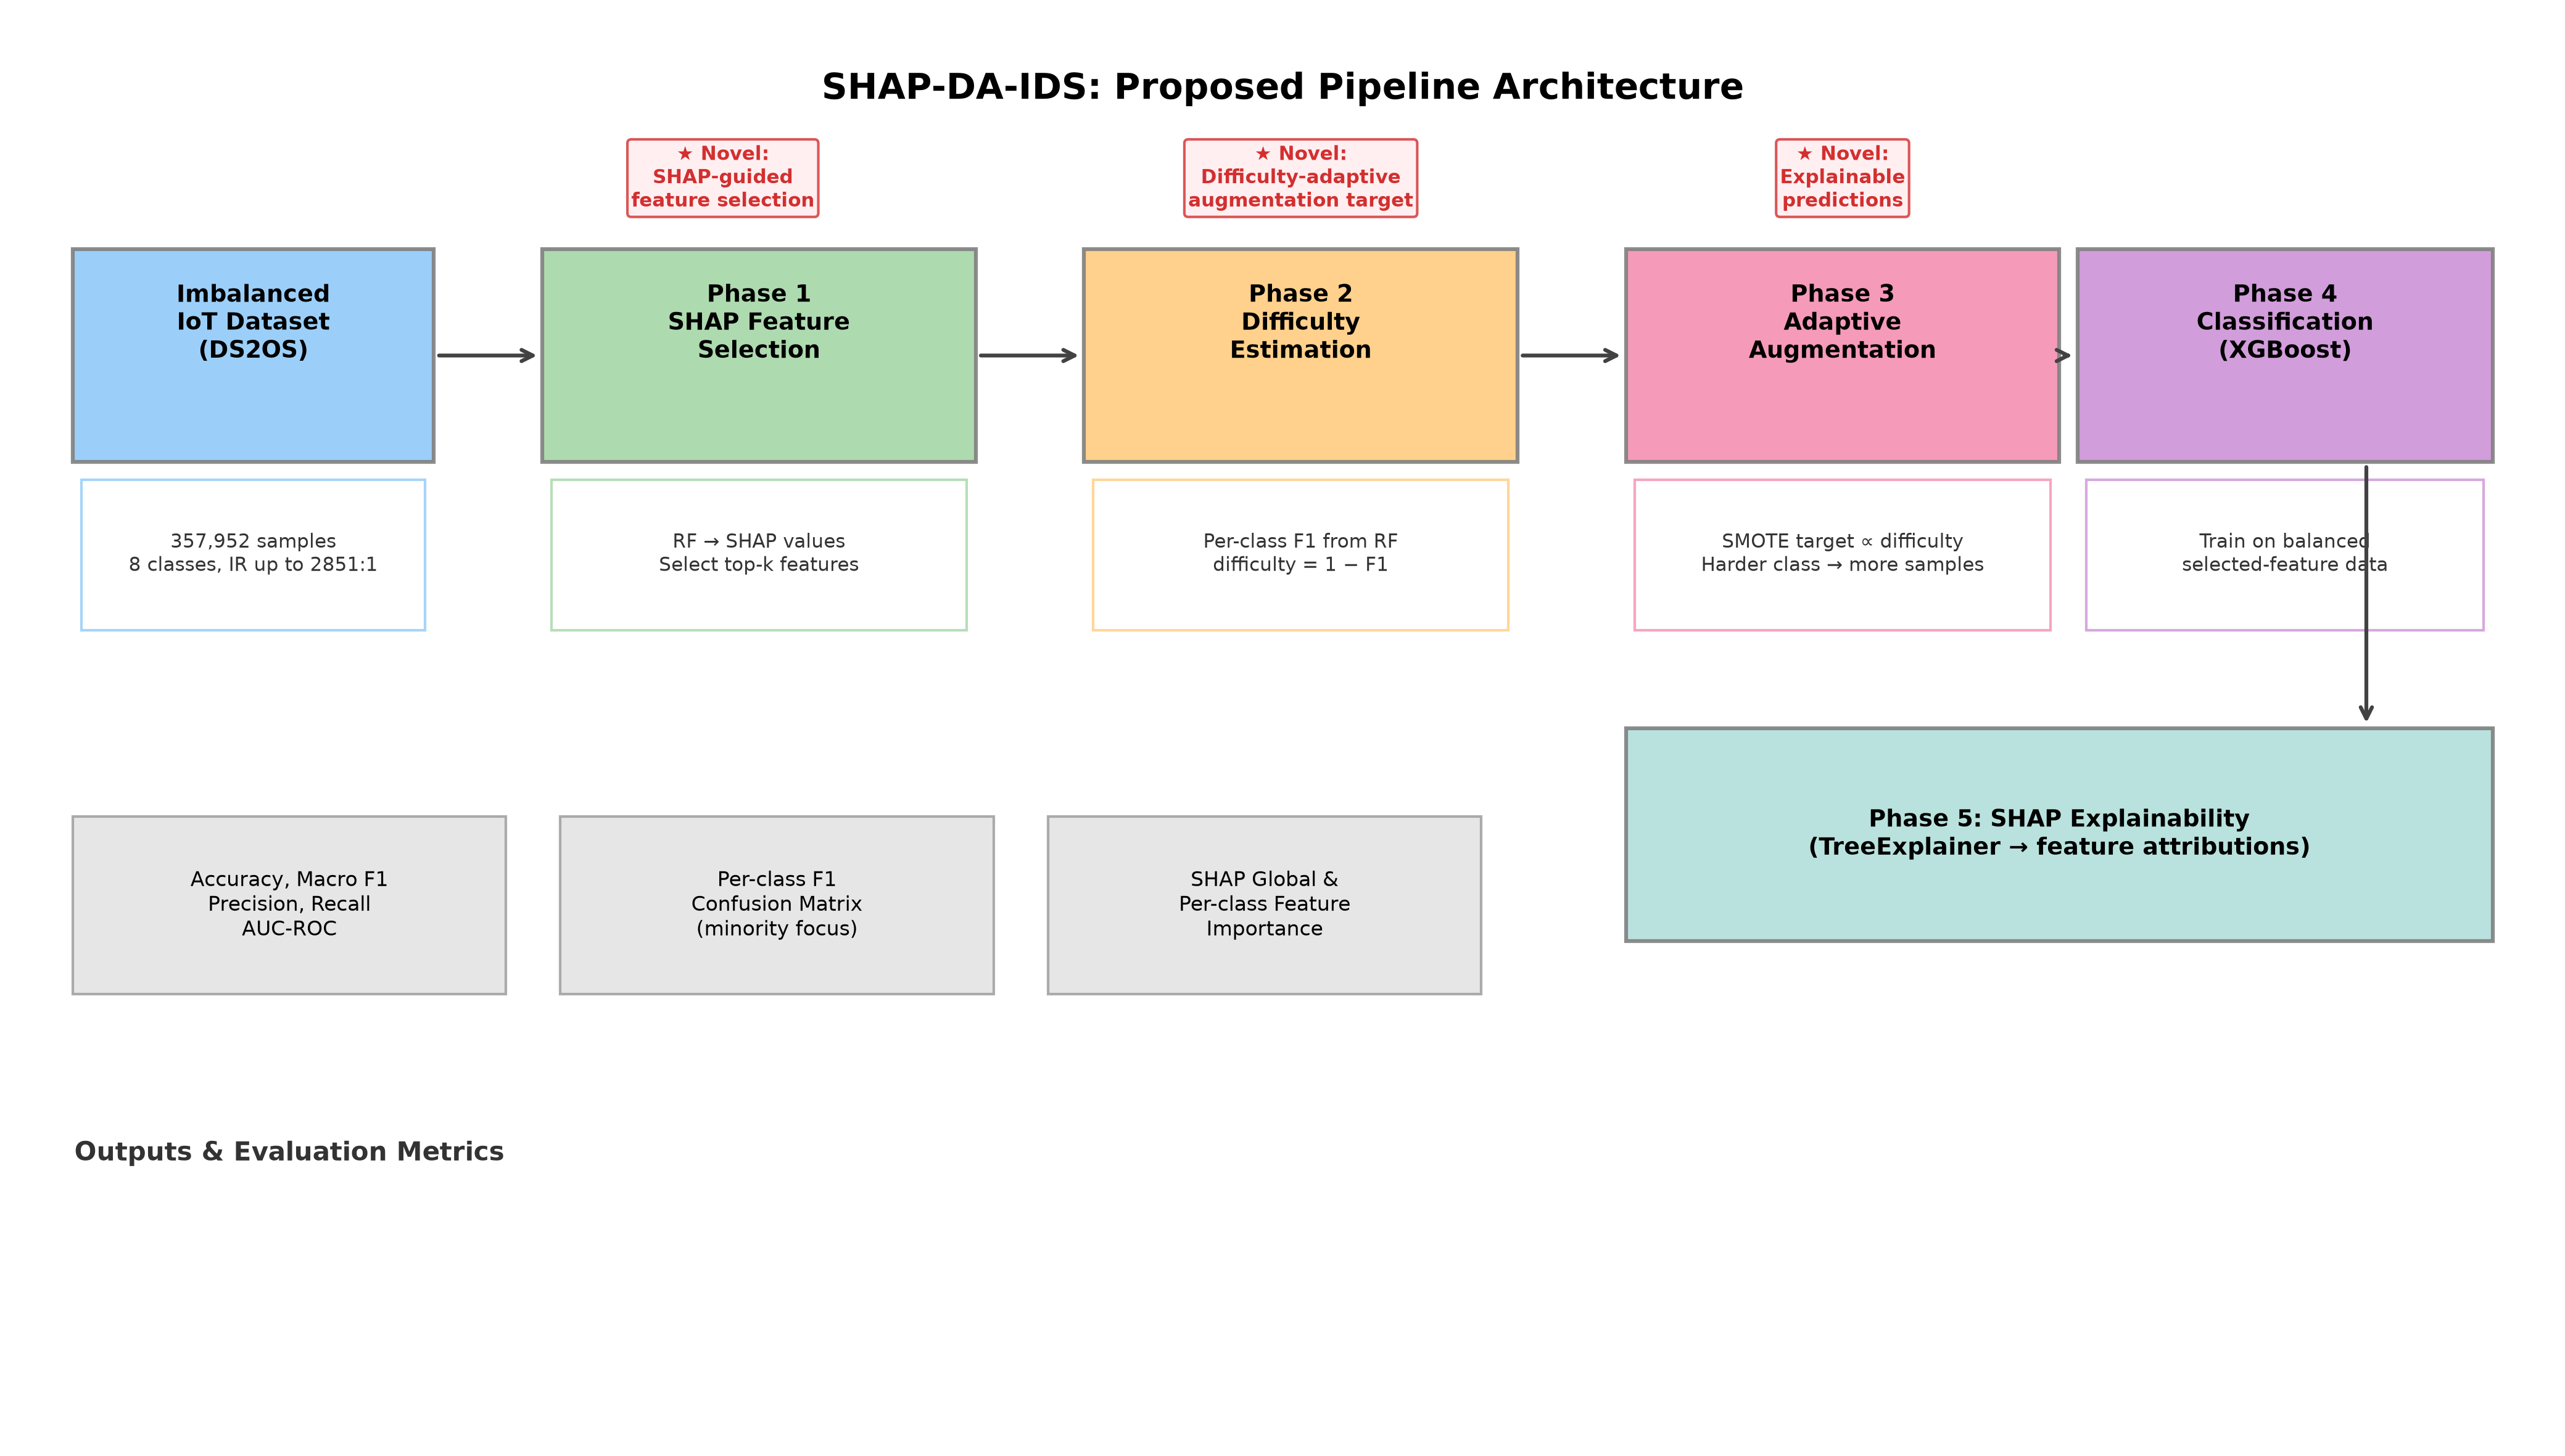
\includegraphics[width=0.92\textwidth]{images/2.png}
\caption{System architecture of the proposed SHAP-DA-IDS framework, illustrating the upstream feature selection, empirical difficulty estimation, adaptive augmentation allocation, and downstream threat attribution.}
\label{fig:architecture}
\end{figure*}

\subsection{Problem Formulation}
Let $\mathcal{D} = \{(x_i, y_i)\}_{i=1}^{N}$ represent an IoT network dataset with $N$ total connection flows. Each flow $x_i \in \mathbb{R}^d$ contains $d$ features, and $y_i \in \{0, 1, \dots, K-1\}$ represents the traffic label. The dataset is dominated by the normal traffic class ($c_{\text{maj}}$), which contains $N_{\text{maj}}$ samples. The remaining $K-1$ attack classes $\mathcal{C}_{\text{min}}$ contain far fewer samples ($N_c \ll N_{\text{maj}}$). The imbalance ratio for any attack class is $\text{IR}_c = N_{\text{maj}} / N_c$.

\subsection{Step 1: SHAP-Guided Feature Selection (SFS)}
Real-world network traces frequently include uninformative or redundant fields. For example, attributes like \texttt{accessedNodeType} often contain missing values in 15\% or more of rows. Passing these directly into an oversampling algorithm inflates the dimensionality without providing useful signals.

To filter the feature space, we first train a preliminary Random Forest classifier $f_{\text{prel}}$ on the training set $\mathcal{D}_{\text{train}}$ using balanced class weights. We then compute the Shapley attribution $\phi_j(x)$ for each feature $j \in \{1, \dots, d\}$ across a background sample $\mathcal{S}_{\text{bg}}$:
\begin{equation}
\phi_j(x) = \sum_{S \subseteq \mathcal{F} \setminus \{j\}} \frac{|S|!(|\mathcal{F}| - |S| - 1)!}{|\mathcal{F}|!} \left[ f(S \cup \{j\}) - f(S) \right]
\label{eq:shapley}
\end{equation}

For multi-class predictions across $K$ classes, the global importance $I_j$ is the mean absolute Shapley value:
\begin{equation}
I_j = \frac{1}{|\mathcal{S}_{\text{bg}}| \cdot K} \sum_{x \in \mathcal{S}_{\text{bg}}} \sum_{k=0}^{K-1} \left| \phi_j^{(k)}(x) \right|
\label{eq:mean_shap}
\end{equation}

We rank features by $I_j$ in descending order and keep the top $m$ features that account for at least 95\% of total importance mass:
\begin{equation}
\frac{\sum_{j=1}^{m} I_{(j)}}{\sum_{j=1}^{d} I_j} \ge 0.95
\label{eq:selection_threshold}
\end{equation}
In our experiments on DS2OS, this step cleanly drops the noisy \texttt{accessedNodeType} feature while preserving the six most informative features.

\subsection{Step 2: Empirical Class Difficulty Estimation}
A key observation in our work is that not all attack classes are equally difficult for a classifier to recognize. Some attacks, like Wrong Setup, exhibit distinct numerical profiles that are easy to spot even with very few examples. Other attacks, like Malicious Control or Data Probing, closely mimic normal traffic patterns and are easily missed.

To quantify this, we run 3-fold cross-validation on $\mathcal{D}_{\text{train}}$ using the feature-selected preliminary model. Let $\text{F1}_c \in [0, 1]$ be the cross-validated F1-score for class $c$. We define the empirical difficulty index $D_c$ as:
\begin{equation}
D_c = 1.0 - \text{F1}_c, \quad \forall c \in \mathcal{C}_{\text{min}}
\label{eq:difficulty}
\end{equation}
A class where the preliminary model scores $\text{F1}=0.02$ has a difficulty of $D_c = 0.98$, indicating that the classifier struggles to find its decision boundary. Conversely, a class with $\text{F1}=0.95$ has $D_c = 0.05$, meaning it is already well separated.

We normalize these difficulty scores across all minority classes:
\begin{equation}
w_c = \frac{D_c}{\sum_{m \in \mathcal{C}_{\text{min}}} D_m}
\label{eq:normalized_weight}
\end{equation}

\subsection{Step 3: Difficulty-Adaptive Augmentation (DAA)}
In original DIFT, the target count for every minority class is clamped to the arithmetic mean of all minority counts:
\begin{equation}
T_c^{\text{DIFT}} = \max\left(N_c, \left\lfloor \frac{1}{|\mathcal{C}_{\text{min}}|} \sum_{m \in \mathcal{C}_{\text{min}}} N_m \right\rfloor\right)
\label{eq:dift_target}
\end{equation}
On DS2OS, this formula produces a target of only 1,144 samples for every attack class, leaving the minority classes outnumbered by Normal traffic ($N_{\text{maj}} = 278,347$) by more than 243 to 1.

Instead, we scale the augmentation target proportionally to class difficulty:
\begin{equation}
T_c^{\text{DAA}} = \min\left( N_{\text{maj}}, \max\left( 2 N_c, N_c + \lfloor w_c \cdot \alpha \cdot N_{\text{maj}} \rfloor \right) \right)
\label{eq:adaptive_target}
\end{equation}
where $\alpha = 0.3$ is a scaling factor that caps the total augmented volume at 30\% of majority traffic. We then generate synthetic points along the minority manifold using $k$-nearest neighbor interpolation:
\begin{equation}
x_{\text{new}} = x_i + \lambda (x_{\text{nn}} - x_i), \quad \lambda \sim \mathcal{U}(0, 1)
\label{eq:smote_interp}
\end{equation}
All oversampling is performed strictly on the training partition $\mathcal{D}_{\text{train}}$ to prevent data leakage into testing.

\subsection{Step 4: Classification with XGBoost}
Once the training set is balanced and filtered, we train an extreme gradient boosting classifier (XGBoost)~\cite{chen2016xgboost}. XGBoost minimizes a regularized multi-class log-loss:
\begin{equation}
\mathcal{L} = \sum_{i=1}^{N_{\text{aug}}} \ell(y_i, \hat{y}_i) + \sum_{t=1}^{T_{\text{trees}}} \left( \gamma T_{\text{leaves}} + \frac{1}{2}\lambda \sum_{j} w_j^2 \right)
\label{eq:xgb_loss}
\end{equation}
The tree regularization term penalizes overly complex branch structures, which helps avoid overfitting on synthetic samples.

\subsection{Step 5: Post-Hoc Threat Attribution}
After the model is trained, we use TreeSHAP~\cite{lundberg2017unified} to explain test-set predictions. For any connection record $x^*$, TreeSHAP decomposes the model's log-odds output into additive feature contributions:
\begin{equation}
g(x^*) = \phi_0^{(c)} + \sum_{j=1}^{m} \phi_j^{(c)}(x^*)
\label{eq:local_explanation}
\end{equation}
This gives network operators a transparent breakdown showing exactly which attributes (such as an illegal operation type or an out-of-range sensor value) led the model to raise an alert.
